\documentclass[a4paper,10pt]{article}
\usepackage[american]{babel}
\usepackage[utf8]{inputenc}
\usepackage[left=2.5cm,top=2cm,right=2.5cm,nohead,nofoot]{geometry}
\usepackage{url}
\usepackage[colorinlistoftodos]{todonotes}
\usepackage{float}
\usepackage{hyperref}

\title{Artifical Intelligence Programming Paradigms\\Assignment 4 : French grammar fragment}
\author{Antoine Carpentier}

\begin{document}

\maketitle

\section{Introduction}

We present a grammar fragment of the French language implemented using Fluid Construction Grammar. The grammar focuses on verb conjugation, omitting verb complements. We chose to restrict our implementation because of the complexity of verb conjugation in French. \\

Our grammar can comprehend and formulate several features of verb phrases such as tense, modality (fact, hypothesis, will, obligation, ability and uncertainty) and the perfect/imperfect aspect. We do not account for other aspects nor passive/active voice. We manage all tenses except for "passé simple" and "passé antérieur" because they fell into disuse in oral form and have approximately the same semantics as "passé composé" and "plus-que-parfait" respectively. We manage all moods except for "gérondif" because it is always used to denote simultaneity with another action and cannot be used alone. \\

The lisp file containing the grammar is "french-vp-grammar.lisp". Annotated examples can be found in the comments at the end of file.

\section{Features of verb conjugation in French}

In French, verbs may have different morphemes depending on person (1, 2 or 3), number (singular or plural), tense, mood and voice. \\

There are 5 past tenses, 1 present tense and 2 future tenses in the indicative mood : \textit{plus-que-parfait}, \textit{passé antérieur}, \textit{imparfait}, \textit{passé simple}, \textit{passé composé}, \textit{présent}, \textit{futur simple} and \textit{futur antérieur}. Of these tenses, 4 are called \textit{composé} (composed) because they are formed with an auxiliary and 4 are \textit{simple} (simple). \\

Composed tenses always denote the perfect aspect while simple tenses always denote imperfection, independantly of mood. The firsts are formed combining an auxiliary conjugated to a simple tense and the past participle of the main verb. Because we only implemented verbs that denote actions (as opposed to verbs that denote states), the auxiliary will always be \textit{avoir} (to have). Composed tenses always denote actions happening before their respective simple form (the one used for the auxiliary). \\

Modality can be expressed in two different ways. First one can add a modal auxiliary conjugated to the right tense before the main verb and conjugate the verb to the infinitive form. These auxiliaries are for example \textit{vouloir} (to want, expressing will), \textit{pouvoir} (to can, expressing ability) and \textit{devoir} (to must, expressing obligation). Second one can use the conditional (expressing hypothesis), subjunctive (expressing uncertainty) or imperative (expressing will) moods that conjugate differently than the indicative.

\section{Implementation}

Our constructions are separated in 5 sets : morphological, lexical, verb phrase, modality and tense. In comprehension they are executed in that order while in formulation there are executed in the order : lexical, verb phrase, modality, tense, morphological. We detail each of these sets in the following subsections. \\

\subsection{Morphological constructions}

Morphological constructions denote each form that a certain lemma (verb in our case) can take and construct syntactical features that are specific to this form. Features are the person, number, tense and mood. Some forms can apply for several persons, tenses or mood, in which case they are all specified. \\

We decided to specifiy each form independently and not construct them from the stem and inflectional morphemes for simplification purposes. It could be enhanced in a future work because verbs can often be grouped by similar patterns of conjugation and few verbs are effectively irregular. \\

Because verbs vary significantly depending on person and number, we only implemented the first person singular but it can be easily improved by adding the right morphological constructions. \\

Constructions for all tenses of the indicative, conditional, subjunctive and imperative moods are available, including the perfect/composed auxiliary \textit{avoir} and the modal auxiliaires \textit{vouloir}, \textit{pouvoir} and \textit{devoir}.

\subsection{Lexical constructions}

Lexical constructions carry the meaning of the verb, which they represent as an event. There is a construction for the perfect auxiliary to indicate the perfect aspect and constructions for each of the modal auxiliaries to indicate their respective modality. \\

\subsection{Verb phrase construction}

The verb phrase construction can be used to extend the grammar in order to add complements. It is not used here as we only implemented verb conjugation except to change the semantic class of the verb to a predicating expression.

\subsection{Modality constructions}

Modality constructions are one part of the main constructions in our grammar, the other part being the tense constructions. First there is a construction that manage composed forms. Second there is a construction that manage modal auxiliaries and third there is one construction for each mood a verb phrase can be conjugated to. \\

The \textbf{perfect-cxn} construction matches with a main verb conjugated to the past participle and an auxiliary verb conjugated to any combination of mood and tense except participle. It merges those units in a new unit with semantic class "predicating expression" conjugated to the tense and mood of the auxiliary and the perfect aspect. \\

The \textbf{modal-aux-cxn} construction matches with a main verb conjugated to the infinitive and a modal auxiliary verb conjugated to any combination of tense, mood and aspect. It merges those in a new unit conjugated to the tense, mood and aspect of the auxiliary verb. \\

The \textbf{part-of-phrase} dummy feature ensures that only one of the \textbf{perfect-cxn} and \textbf{modal-aux-cxn} constructions is run as an auxiliary cannot be both modal and perfect. \\

The last 4 constructions of this set match with a verb phrase conjugated to respectively the indicative, conditional, sunjunctive and imperative moods. They create the meaning of modality for each of these moods. Because these constructions match with a verb phrase instead of an action, they are always applied after the aspect and modal auxiliary constructions. \\

The \textbf{mood-phrase} dummy feature ensures that only one mood construction is applied on each verb phrase. \\

\subsection{Tense constructions}

Finally the tense constructions match a verb phrase conjugated to a specific tense and merge the meanings of time, namely the origo and the situation of the action on the timeline compared to it. These constructions apply to any mood or aspect. 

There are only 3 tense constructions because when combined with the two values of aspect (perfect/imperfect) it can express the 6 tenses we are interested in. The figures \ref{indicativetenses}, \ref{conditionaltenses} and \ref{subjunctivetenses} show the matching between tenses in French and our constructions for respectively the indicative mood, the conditional and imperative moods and the subjunctive mood. These constructions make sense because as we said earlier the perfect aspect in French verbs always denotes an action happening earlier than its corresponding imperfect action. \\

We thus have two aspects for the past tense : the past imperfect corresponds to the \textit{imparfait} and denotes unachieved recent actions while the past perfect correspond to the \textit{plus-que-parfait} and denotes finished earlier actions. The same holds for the present and future tenses and in any mood. \\


\begin{figure}[!h]
    \centering
    \begin{tabular}{c|c|c|c}
        & \textbf{past} & \textbf{present} & \textbf{future} \\\hline
        \textbf{perfect} & plus-que-parfait & passé composé & futur antérieur \\\hline
        \textbf{imperfect} & imparfait & présent & futur simple \\    
    \end{tabular}
    \caption{Tenses in indicative mood based on aspect}
    \label{indicativetenses}
\end{figure}

\begin{figure}[!h]
    \centering
    \begin{tabular}{c|c}
        & \textbf{present} \\\hline
        \textbf{perfect} & présent \\\hline
        \textbf{imperfect} & passé \\    
    \end{tabular}
    \caption{Tenses in conditional and imperative mood based on aspect}
    \label{conditionaltenses}
\end{figure}

\begin{figure}[!h]
    \centering
    \begin{tabular}{c|c|c|c}
        & \textbf{past} & \textbf{present} \\\hline
        \textbf{perfect} & plus-que-parfait & passé \\\hline
        \textbf{imperfect} & imparfait & présent \\    
    \end{tabular}
    \caption{Tenses in subjunctive mood based on aspect}
    \label{subjunctivetenses}
\end{figure}

\section{Results and discussion}

Our examples are all based on the verb \textit{atterrir} (to land). \\

The figures \ref{application-process-FA} and \ref{meaning-FA} show the comprehension of the \textit{futur antérieur} "aurai atterri". We see that it corresponds to the indicative future perfect. The \textbf{past-cxn} construction was tried for the past participle but it fails because the verb phrase unit is conjugated to the tense of the auxiliary, that is future in this case. The meaning clearly expresses a perfect action situated after the present the indicates a fact. The resulting structure being too large to display, please see the code for further information. \\

The figures \ref{application-process-mod-aux-subj-PQP} and \ref{meaning-mod-aux-subj-PQP} show the comprehension of the \textit{subjonctif plus-que-parfait} with auxiliary \textit{devoir} "eusse dû atterrir". We see that the tense, aspect and mood are applied on the auxiliary and that the main verb (conjugated to the infinitive) only carries its lexical meaning. \\

The figures \ref{application-process-present}, \ref{meaning-present} and \ref{resulting-structure-present} show the comprehension of the \textit{présent} "atterris" which can be either imperative or indicative. The ambiguity can be noticed in the application process where any of the imperative and indicative moods can be chosen and it only depends on which is selected first. \\

The figure \ref{application-process-mod-aux-subj-PQP-form} show the application process when formulating past perfect with modalities obligation and uncertainty. The first modality being expressed with the modal auxiliary \textit{devoir} and the second with the subjunctive mood, they can be combined in a verb phrase. The result is "eusse dû atterrir". We can see that in formulation there is no ambiguity if sufficent information is given.

\begin{figure}[!h]
    \centering
    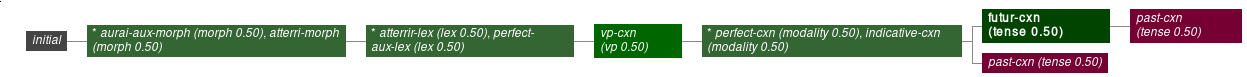
\includegraphics[width=\textwidth]{application-process-FA.png}
    \caption{Application process when comprehending "aurai atterri"}
    \label{application-process-FA}
\end{figure}

\begin{figure}[!h]
    \centering
    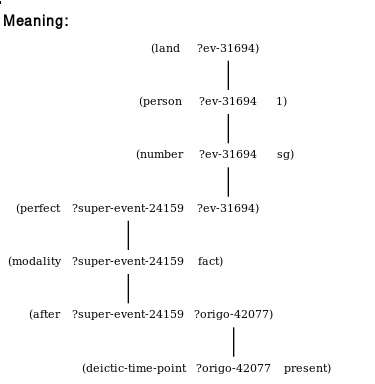
\includegraphics[width=200px]{meaning-FA.png}
    \caption{Meaning obtained when comprehending "aurai atterri"}
    \label{meaning-FA}
\end{figure}

% \begin{figure}[!h]
%     \centering
%     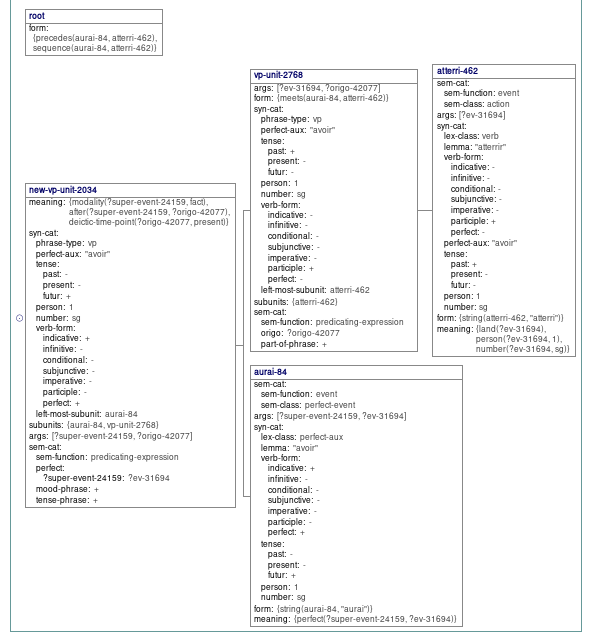
\includegraphics[width=\textwidth]{resulting-structure-FA.png}
%     \caption{Resulting structure when comprehending "aurai atterri"}
%     \label{resulting-structure-FA}
% \end{figure}

\begin{figure}[!h]
    \centering
    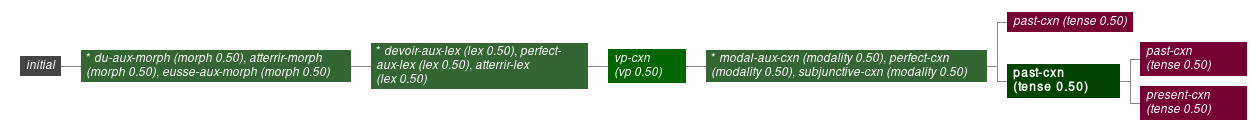
\includegraphics[width=\textwidth]{application-process-mod-aux-subj-PQP.png}
    \caption{Application process when comprehending "eusse dû atterrir"}
    \label{application-process-mod-aux-subj-PQP}
\end{figure}

\begin{figure}[!h]
    \centering
    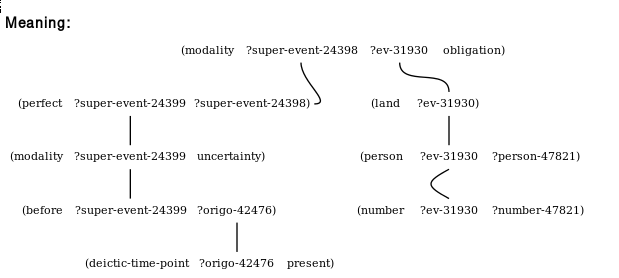
\includegraphics[width=400px]{meaning-mod-aux-subj-PQP.png}
    \caption{Meaning obtained when comprehending "eusse dû atterrir"}
    \label{meaning-mod-aux-subj-PQP}
\end{figure}

% \begin{figure}[!h]
%     \centering
%     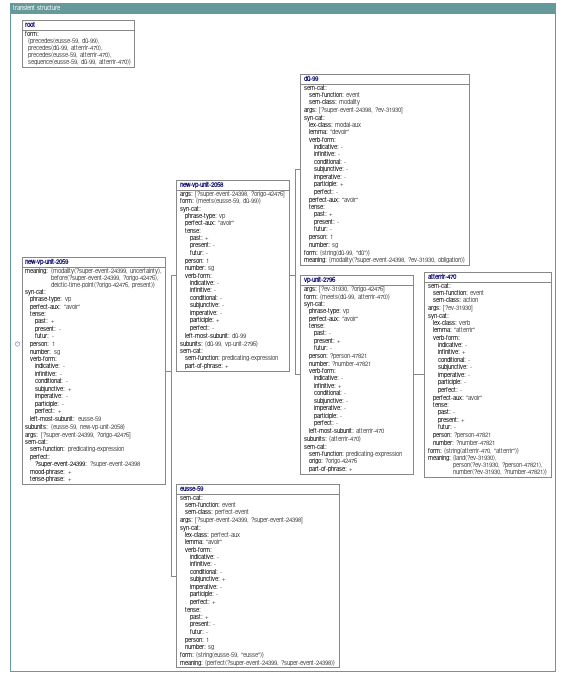
\includegraphics[width=\textwidth]{resulting-structure-mod-aux-subj-PQP.png}
%     \caption{Resulting structure when comprehending "eusse dû atterrir"}
%     \label{resulting-structure-mod-aux-subj-PQP}
% \end{figure}

\begin{figure}[!h]
    \centering
    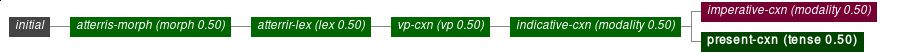
\includegraphics[width=\textwidth]{application-process-present.png}
    \caption{Application process when comprehending "atterris"}
    \label{application-process-present}
\end{figure}

\begin{figure}[!h]
    \centering
    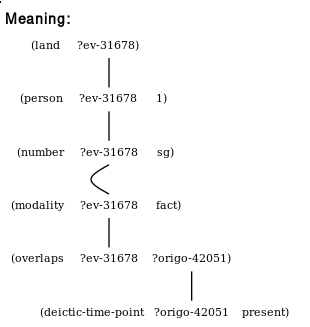
\includegraphics[width=200px]{meaning-present.png}
    \caption{Meaning obtained when comprehending "atterris"}
    \label{meaning-present}
\end{figure}

\begin{figure}[!h]
    \centering
    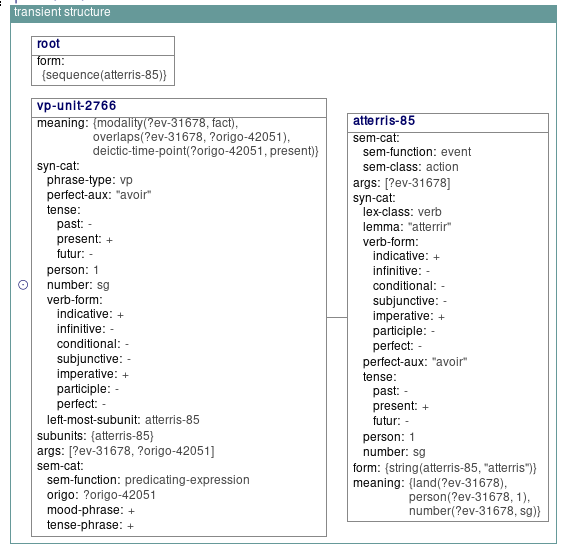
\includegraphics[width=\textwidth]{resulting-structure-present.png}
    \caption{Resulting structure when comprehending "atterris"}
    \label{resulting-structure-present}
\end{figure}

\begin{figure}[!h]
    \centering
    
\includegraphics[width=\textwidth]{application-process-mod-aux-subj-PQP-form.png}
    \caption{Application process when formulating past perfect with modalities obligation and uncertainty}
    \label{application-process-mod-aux-subj-PQP-form}
\end{figure}

Our grammar is bi-directional in the sense that it can produce any utterance with a properly constructed meaning and it always returns back the good utterance when using the \textbf{comprehend-and-formulate} function. If the meaning is not defined enough, several utterances are possible. \\

We do not get many solutions per sentence because we intentionally reduced the number of morphemes by implementing only the first person singular. An example of ambiguous comprehension is the present of the indicative and imperative moods that share the same utterance. There cannot be ambiguous formulation as long as tense, modality and aspect are specified. Several modalities can be expressed at the same time using both a modal auxiliary and the mood. \\

Extensions to our grammar could include the \textit{passé simple} and \textit{passé antérieur}, completing morphemes for every person and number and adding auxiliaires that modify the aspect of the verb such as \textit{commencer à} (start to) that denotes the inchoative aspect. The latter would need to extend the grammar to include prepositions. We could also construct lemma using stem and morphemes and categories of verbs that conjugate in the same way. \\

\section{Conclusion}

What we learnt from this work is that French verb conjugation is difficult for two reasons. First modality can be expressed by moods or using auxiliary verbs. Second there are different morphemes for almost every combination of person, number, tense and mood and they might collide. \\

It is also simple in the sense that the perfect aspect is completely reflected in the system of simple and composed tenses and that the same system can help to construct tenses in a structured way. \\

We implemented a large part of the verb conjugation in French, missing only the passive/active voice and the state denoting verbs to be used in practical applications.

\end{document}

